\chapter{Покомпонентные методы и вычислительные оптимизации}

\section{Постановки задач}

%Рассматривается трехмерная структурная обратная задача гравиметрии о нахождении поверхностей раздела сред по известным скачкам плотности и гравитационному полю, измеренному на некоторой площади земной поверхности.
%Рассмотрим уравнение гравиметрии для модели двуслойной среды в декартовой системе координат с осью $z$, направленной вниз 
%\begin{equation}\label{equ_grav2l}
%\begin{aligned}
%\gamma\Delta\sigma\frac{1}{4\pi} \bigg\{ \iint_{D} \frac{1}{[(x-x')^2+(y-y')^2+H^2]^{1/2}}dx'dy' \\
%- 
%\iint_{D} \frac{1}{[(x-x')^2+(y-y')^2+u^2(x',y')]^{1/2}}dx'dy'\bigg\}=\Delta g(x,y),
%\end{aligned} 
%\end{equation}
%где $\gamma$ --- гравитационная постоянная, $\Delta\sigma=\sigma_2-\sigma_1$ --- скачок плотности на поверхности раздела сред, описываемой функцией $u(x,y)$ и подлежащей определению, $f(x,y)$ --- аномальное гравитационное поле, вызванное отклонением поверхности от асимптотической плоскости $z=H$ для искомого решения $u(x,y)$ (рис.~\ref{fig:twolayergrav}). 
%\begin{figure}
%	\centering
%	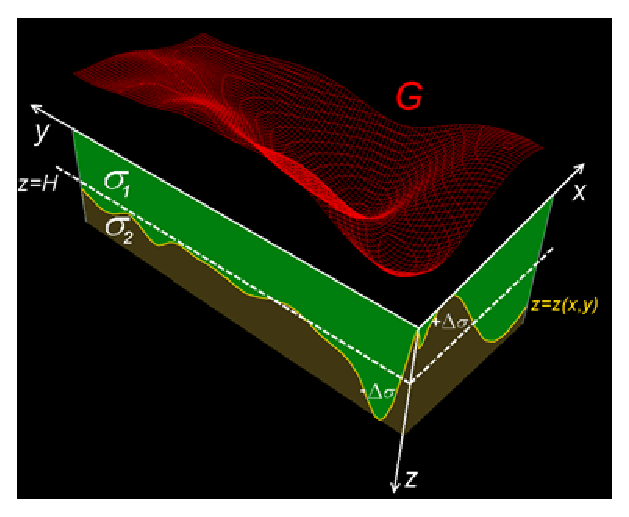
\includegraphics[height=6.0cm]{Twolaymodgrav}
%	\caption{Модель двуслойной среды в задаче гравиметрии.}
%	\label{fig:twolayergrav}
%\end{figure}
%Запишем $\eqref{equ_grav2l}$ в виде операторного уравнения
%\begin{equation}\label{equ_2lop}
%[A(u)](x,y)=-\iint_{D} \frac{1}{[(x-x')^2+(y-y')^2+u^2(x',y')]^{1/2}}dx'dy'=f(x,y),
%\end{equation}
%где $f(x,y)=\Delta g(x,y) 4\pi/\gamma\Delta\sigma - A(H)$. Тогда производная оператора $A$ в точке $u^0(x,y)$ определяется формулой
%$$ [A'(u^0)]h=\iint_{D} \frac{u^0(x',y')h(x',y')}{[(x-x')^2+(y-y')^2+(u^0(x',y'))^2]^{3/2}}dx'dy', $$
%Уравнение (\ref{equ_2lop}) является интегральным уравнением Урысона (так как неизвестная функция $u(x,y)$ входит в ядро оператора нелинейно) I рода, следовательно, относится к классу некорректных задач.
%
%После дискретизации интегрального уравнения $\eqref{equ_2lop}$ двумерным аналогом формулы прямоугольников с равномерной сеткой по каждой переменной с шагом $\Delta x$, $\Delta y$, получаем систему нелинейных уравнений относительно неизвестного вектора $u_{ji}=u(x_j,y_i)\quad (j=1,2,...,N, i=1,2,...,M)$, которая в векторно-матричном виде может быть записана следующим образом
%\begin{equation}\label{equ_snle}
%A_n(u_n)=f_n,
%\end{equation}
%где $u_n$, $f_n$ --- векторы размерности $n=N\times M$. Дискретный аналог производной $A'(u^0)$ принимает форму
%\begin{equation}\label{op_grav_disc_form}
%[A'_n(u_n^0)h_n]_{k,l}=\sum\limits_{i=1}^{M}\sum\limits_{j=1}^{N}
%\Delta x\Delta y\frac{u^0_{ji}h_{ji}}{[(x_k-x'_j)^2+(y_l-y'_i)^2+(u^0_{ji})^2]^{3/2}},
%\end{equation}
%где при $u_n=u_{n}^{0}$ --- const $A'_n(u_n^0)$ --- симметричная матрица, компоненты которой вычисляются по формуле $\eqref{op_grav_disc_form}$.

Рассмотрим уравнение гравиметрии для модели многослойной среды. 

Предполагается, что нижнее полупространство состоит из нескольких слоев постоянной плотности $\Delta\sigma_l(l=1,..,L)$, разделенных искомыми поверхностями $S_l$, где $L$~--- число границ раздела (рис.~\ref{fig:multlayer}). Гравитационный эффект от такого полупространства равен сумме гравитационных эффектов от всех поверхностей раздела.
\begin{figure}
	\centering
	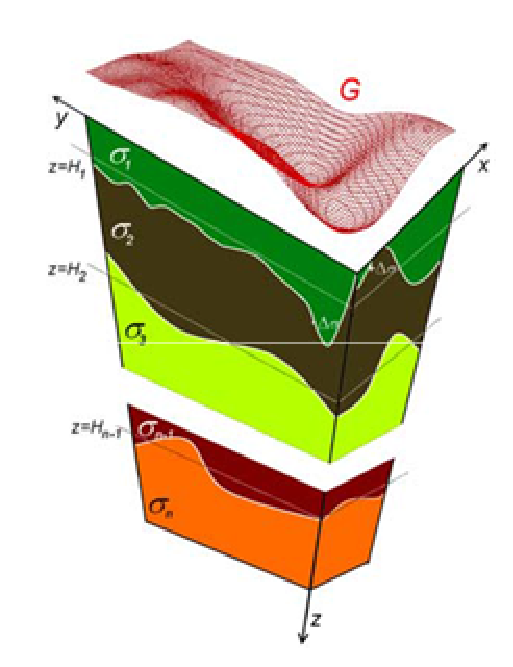
\includegraphics[height=6.0cm]{MultilayerModel}
	\caption{Модель многослойной среды.}
	\label{fig:multlayer}
\end{figure}
Пусть поверхности раздела задаются уравнениями $u_l(x,y)$, скачки плотности на них равны $\Delta\sigma_l$. поверхности имеют горизонтальные асимптотические плоскости $u_l=H_l$, т.е. $$\lim_{|x|,|y|\to\infty}|u_l(x,y)-H_l|=0.$$ Функции $u_l(x,y)$, $u=(u_1(x,y), .., u_L(x,y))$, описывающие искомые поверхности раздела сред, удовлетворяют операторному уравнению
\begin{equation}\label{equ_grav}
\begin{aligned}
A(u)=\sum_{l=1}^{L}f\Delta\sigma_l\frac{1}{4\pi}\iint_D\bigg\{\frac{1}{[(x-x')^2+(y-y')^2+u_l^2(x,y)]^{1/2}} \\
-\frac{1}{[(x-x')^2+(y-y')^2+H_l^2]^{1/2}}\bigg\}=\Delta g(x',y'),
\end{aligned}
\end{equation}
где $f$~---~гравитационная постоянная, $\Delta\sigma_l(l=1,..,L)$ скачки плотности, $\Delta g(x',y')=\sum_{l=1}^{L}g_l$~--- суммарное аномальное гравитационное поле. 

Предварительная обработка гравитационных данных с выделением аномального поля из измеренных гравитационных данных выполняется по методике  \cite{MarPrut2003}. Задача является недоопределенной, так как мы ищем несколько функций $u_l(x,y)$ по заданной функции $\Delta g(x',y')$. Поэтому необходимо использовать весовые множители, которые могут быть найдены по формулам из \cite{AkMarMis2013}:
$$F=[F_1, F_2, ..., F_L]=(f_1, f_2, ..., f_{M\times L}, ..., f_{L\times M\times N})$$
$$\to (w_1, w_2, ..., w_{L\times M\times N}),$$
\begin{equation}\label{weght_fact_formula}
w_i=\frac{|f_i|^\beta}{\max\limits_{i} |f_i|^\beta}, \quad \beta>1,
\end{equation}
где $F_l (l=1, 2, ..., L)$ --- аномальные гравитационные поля, создаваемые гравитирующими массами, находящимися на соответствующих глубинах $H_l$ и разделенных границами раздела $S_l(l=1, 2, ..., L)$.

После дискретизации уравнения $(\ref{equ_grav})$ на сетке $n=M\times N$ с заданной правой частью $\Delta g(x',y')$ и аппроксимации интегрального оператора $A(u)$ по квадратурным формулам, получаем вектор правой части $F(x',y')$ размера  $M\times N$, вектор решения $u(x,y)=[u_1(x,y),..,u_L(x,y)]$ размерности $L\times M\times N$, полученный конкатенацией векторов решений, соответствующих $l$-й границе раздела, матрицу производной оператора $A'(u)$ размерности $(M\times N)\times(L\times M\times N)$, полученной приписыванием справа к матрице производной $A'(u^l)$ в точке $u^l$ матрицы $A'(u^{l+1})$, где
\begin{equation}\label{op_grav_disc_form_mult}
[A'(u_n^l)h_n]_{k,m}=\sum\limits_{i=1}^{M}\sum\limits_{j=1}^{N}
\Delta x\Delta y\frac{u^l_{ij}h^l_{ij}}{[(x_k-x'_i)^2+(y_m-y'_j)^2+(u^l_{ij})^2]^{3/2}},
\end{equation} и систему нелинейных уравнений  
\begin{equation}\label{snl_equ}
A_n[u]=F_n.
\end{equation}
Критерием останова итераций выбрана относительная норма невязки $\|A_n(u^k)-F_n\|/\|F_n\|$ точного и численного решений при достаточно малом $\varepsilon$.

%Уравнение магнитометрии при тех же предположениях, что и в задаче гравиметрии для двухслойной среды, имеет вид:
%\begin{equation}\label{equ_magn}\begin{aligned}
%\Delta J  \bigg\{&\iint_{D} \frac{H}{[(x-x')^2+(y-y')^2+H^2]^{3/2}}dx'dy' \\
%- &\iint_{D} \frac{u(x',y')}{[(x-x')^2+(y-y')^2+u^2(x',y')]^{3/2}}dx'dy' \bigg\}=\Delta G(x,y),
%\end{aligned} \end{equation}
%где $\Delta J$ -- усредненный скачок $z$-компоненты вектора намагниченности, $z=H$ -- асимптотическая плоскость, $u(x,y)$ -- функция, описывающая аномальное поле, $z=u(x,y)$ -- искомая функция, описывающая поверхность раздела сред с различными свойствами намагниченности (рис.~\ref{fig:twolayermag}). 
%\begin{figure}
%	\centering
%	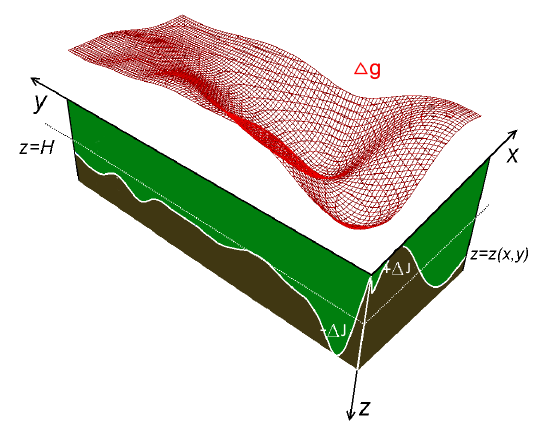
\includegraphics[height=6.0cm]{Twolaymodmag}
%	\caption{Модель двуслойной среды в задаче гравиметрии.}
%	\label{fig:twolayermag}
%\end{figure}
%Уравнение $\eqref{equ_magn}$ можно переписать в форме
%\begin{equation}\label{equ_magn_op}
%[D(u)](x,y)= \iint_{D} \frac{u(x',y')}{[(x-x')^2+(y-y')^2+u^2(x',y')]^{3/2}}dx'dy'=F(x,y),
%\end{equation}
%где $F(x,y)=D(H)-\Delta G(x,y)/\Delta J$, тогда производная оператора $D$ в точке $u^0(x,y)$ определится формулой
%$$ [A'(u^0)]h=\iint_{D} \frac{(x-x')^2+(y-y')^2-2(u^0(x',y'))^2}{[(x-x')^2+(y-y')^2+(u^0(x',y'))^2]^{5/2}}h(x',y')dx'dy'. $$
%
%После дискретной аппроксимации подобно задаче гравиметрии уравнения $\eqref{equ_magn_op}$, приходим к системе нелинейных уравнений
%\begin{equation}\label{equ_snle_mag}
%D_n(u_n)=F_n
%\end{equation}
%относительно вектора $u_n \quad (n=N\times M)$ с компонентами $u_{ij}\quad (i=1,2,...,N, j=1,2,...,M)$, при этом компоненты производной оператора $D_n$ в точке $u_{n}^{0}$ вычисляются по формуле
%\begin{equation}\label{deriv_op_mag}
%	[D'_n(u_{n}^{0})h_n]_{k,l}=\sum\limits_{i=1}^{N}\sum\limits_{j=1}^{M}
%	\Delta x\Delta y\frac{(x_k-x'_j)^2+(y_l-y'_i)^2-2(u_{ji}^0)^2}{[(x_k-x'_j)^2+(y_l-y'_i)^2+(u_{ji}^0)^2]^{5/2}}h_{ji}, 
%\end{equation}
%причем при $u_{n}^{0}=\{u^0(x'_j, y'_i), 1\le j\le M, 1\le i\le N\}=const$, $D'_n(u_n^0)$ -- симметричная матрица.

\section{Вычислительная оптимизация метода Ньютона}

Для задач (\ref{equ_snle}), (\ref{equ_snle_mag}) можно отметить, что элементы матриц $A'(u^0)$ (\ref{op_grav_disc_form}), (\ref{deriv_op_mag}) принимают наибольшие значения при малых значениях $(x-x')$ и $(y-y')$ (Рис. \ref{fig:matrixscheme}).
\begin{figure}
	\centering
	\includegraphics[height=6.0cm]{Matrix}
	\caption{Схема матрицы производной оператора $A$ в задачах грави- магнитометрии в двухслойной среде}
	\label{fig:matrixscheme}
\end{figure}
Однако при возрастании глубины $H$ асимптотической плоскости по сравнению с площадью $D$ --- размером сетки, выраженная <<ленточность>> матрицы производной оператора теряется.

Поэтому в структурных обратных задачах грави- магнитометрии при небольших относительно размера сетки глубинах $H$ при решении итерационными методами без существенной потери точности можно не учитывать значения элементов, отстоящих от диагонали далее, чем на  $\beta$-ю часть  размерности матрицы производной, то есть те значения $a_{ij}$, для которых  $j \in \{i-h(\beta),..i+h(\beta)\} $, где $h(\beta)$ --- полуширина ленты матрицы, $i, j$ --- индекс элемента. Данный подход позволяет существенно уменьшить количество вычислительных операций, перейдя от плотно заполненных матриц к матрицам ленточного вида.

В данной работе приведены результаты расчетов модельных задач гравиметрии и магнитометрии в двухслойной среде методами Ньютона и модифицированным его вариантом.

\section{Покомпонентный метод типа Ньютона}

Запишем исходное операторное уравнение (1.1) в виде:
$$P(u)=A(u)-f,$$
где $A(u)=\int_{a}^{b}\int_{c}^{d}K(x,y, x',y',u^k(x,y))dxdy$ --- интегральный оператор задачи гравиметрии (\ref{equ_grav2l}).

Итерации в методе Ньютона строятся по схеме
$$A'(u^k)(\Delta u^k)=-(A(u^k)-f),$$ где $\Delta u^k=u^{k+1}-u^k$.
То есть, для задачи гравиметрии
$$f\Delta\sigma\int_{a}^{b}\int_{c}^{d}K'_u(x,y, x',y',u^k(x,y))\Delta u^k dxdy=[A(u^k)](x',y')-f(x',y').\eqno(4.3)$$
В задаче гравиметиии на изменение гравитационного поля в правой части (4.3) наибольшее значение оказывает отклонение искомой функции точного решения $z$ от асимптотической плоскости в точке $(x',y')$. Тогда можем записать
\begin{equation}\label{comp_newt_meth_step1}
f\Delta\sigma(\Delta u^k)\int_{a}^{b}\int_{c}^{d}K'_u(x,y, x',y',u^k(x,y)) dxdy=A(u(x',y'))-f(x',y').
\end{equation}
Таким образом, величина поправки $\Delta u^k$ может быть получена как
$$\Delta u^k=\bigg[[A(u)](x',y')-f(x',y')\bigg]\bigg/f\Delta\sigma\int_{a}^{b}\int_{c}^{d}K'_u(x,y, x',y',u^k(x,y)) dxdy,$$ 
итерации осуществляются по схеме:
\begin{equation}\label{comp_newt_meth}
u^{k+1}(x',y')=u^k(x',y')-\frac{1}{\psi^k(x',y')}([A(u^k)](x',y')-f(x',y')),$$
где $$\psi^k(x',y')=f\Delta\sigma\int_{a}^{b}\int_{c}^{d}K'_u(x,y, x',y',u^k(x,y)) dxdy.
\end{equation}
В дискретной записи итерационный процесс запишется
$$u_{k,m}^{k+1}=u_{k,m}^k-\frac{1}{\psi_{k,m}^k}([A_n(u^k)]_{k,m}-f_{k,m}),\quad 1\le k \le M, \quad 1\le m \le N,$$
где $$\psi_{k,m}^k=f\Delta\sigma\sum\limits_{i=1}^{M}\sum\limits_{j=1}^{N}
\Delta x\Delta y\frac{u_{ij}}{[(x_k-x'_j)^2+(y_l-y'_i)^2+(u_{ij})^2]^{3/2}}.$$
Эту сумму $\psi_{k,m}^k$ можно интерпретировать как сумму элементов $(k\times M + l)$-й строки матрицы производной $A'_n(u_n^k)$.

Предложенный метод позволяет существенно упростить вычисления по сравнению с методом Ньютона. Вместо вычисления обратной матрицы в методе Ньютона можно вычислить вектор, состоящий из сумм элементов строк матрицы и использовать его компоненты для восстановления соответствующей компоненты вектора решения $u_n^k$. Вычислительная сложность метода Ньютона составляет $O(n^2)$, если для обращения матрицы производной $A'_n(u_n)$ использовать методы градиентного типа, в то время как вычислительная сложность покомпонентного метода $O(n)$.

\section{Покомпонентный метод типа Левенберга---Марквардта}

Для решения задач (\ref{equ_grav2l}), (\ref{equ_grav}) предлагается метод покомпонентного типа, основанный на идее метода Левенберга---Марквардта. 

Для аппроксимации решения уравнения (\ref{equ_2lop}) метод Левенберга---Марквардта (МЛМ) имеет вид:
\begin{equation}
u^{k+1}=u^k-\gamma[A'(u^k)^*A'(u^k)+\alpha I]^{-1} A'(u^k)^*(A(u^k)-f_\delta),
\end{equation}
где $A'(u^k)^*$ --- оператор, сопряженный к производной оператора $A$ задачи $A'(u)$, $\alpha>0$~--~параметр регуляризации, $\|f-f_\delta\|\le \delta.$
 
В работах В.В. Васина \cite{Vasin_2012}, \cite{VasPer_2011} был исследован метод Левенберга---Марквардта
\begin{equation}\label{LM_Vasin}
u^{k+1}=u^k-\gamma[A'(u^k)^*A'(u^k)+\bar{\alpha} I]^{-1} [A'(u^k)^*(A(u^k)-f_\delta)+\alpha (u-u^0)]
\end{equation} и его модифицированный вариант
\begin{equation}\label{LM_modif_Vasin}
u^{k+1}=u^k-\gamma[A'(u^0)^*A'(u^0)+\bar{\alpha} I]^{-1} [A'(u^k)^*(A(u^k)-f_\delta)+\alpha (u-u^0)]
\end{equation} для решения регуляризованного уравнения
$$A'(u)^*(A(u)-f_\delta)+	\alpha (u-u^0)=0,$$
где $\gamma$ --- демпфирующий множитель, $u^0$ --- некоторое приближение к $u_\alpha$, $\alpha>0$. На основании выводов, сделанных М.Ю. Кокуриным \cite{Kok_2010} о свойствах градиента $\Phi_\alpha '(u)$ тихоновского функционала $$\Phi_\alpha(u)=(1/2)(\|A(u)-f_\delta\|^2+\alpha\|u-\xi\|^2)$$ было установлено, что при выборе параметров $\bar{\alpha}$, $\alpha$, $\gamma$ имеет место сильная сходимость итераций (\ref{LM_Vasin}), (\ref{LM_modif_Vasin}) к регуляризованному решению $u_\alpha$.

По аналогии с покомпонентным методом типа Ньютона (\ref{comp_newt_meth}), можно выполнить прием вынесения значимой компоненты за знак интегрального оператора, как в (\ref{comp_newt_meth_step1}) и запишем итерационную последовательность восстановления каждой из неизвестных границ $u_l$
\begin{equation}\label{comp_lm_meth}
u_l^{k+1}=u_l^k-\gamma\frac{1}{\varphi_l}\Lambda[ A'(u_l^k)^T(A(u^k)-f_\delta)+\alpha (u_l^k-u_l^0)],
\end{equation}
где $l$ -- номер границы раздела, $l=1,..,L$, $\Lambda$ --- диагональная матрица, состоящая из весовых множителей, 
\begin{equation*}
\begin{aligned}
\varphi_l=\bigg[ f\Delta\sigma\int_{a}^{b}\int_{c}^{d}
K'_u(x',y', x, y, u_l^k(x,y))dx'dy'\bigg] \notag \\ \times\bigg[f\Delta\sigma\int_{a}^{b}\int_{c}^{d}K'_u(x,y, x',y',u_l^k(x,y))dxdy\bigg], 
\end{aligned}
\end{equation*} 
где $K'_u(x',y', x, y, u_l^k(x,y))$ --- функция ядра, транспонированного к ядру $K'_u(x,y,$ $ x',y',u^k(x,y))$. Величина $\varphi_l$ зависит от $u_l^k$.
Итерационный процесс (\ref{comp_lm_meth}) перепишем в дискретной форме
\begin{equation}\label{comp_lm_meth_disc}
u_{l,i}^{k+1}=u_{l,i}^k-\gamma\frac{1}{\varphi_{l,i}}w_{l,i}\bigg[ \{A'(u_l^k)^T(A(u^k)-f_\delta)\}_i+\alpha (u_{l,i}^k-u_{l,i}^0)\bigg],
\end{equation}
где $w_{l,i}$ --- $i$-й весовой множитель, зависящий от $l$-й границы раздела,
\begin{equation*}
\begin{aligned}
\varphi_{l,i}=\bigg[ f\Delta\sigma\sum\limits_{k=1}^{N}
\sum\limits_{m=1}^{M}
K'_u(x'_k,y'_m, \{x, y\}_i, u_{l,i}^k) \Delta x' \Delta y'\bigg] \notag \\ \times\bigg[f\Delta\sigma\sum\limits_{k=1}^{N}
\sum\limits_{m=1}^{M}K'_u(x_k,y_m, \{x',y'\}_i,u_l^k(x_k,y_m))\Delta x \Delta y\bigg]. 
\end{aligned}
\end{equation*}

Преимущества покомпонентного метода типа Левенберга---Марквардта в низкой вычислительной сложности. Здесь не требуется вычисления матрицы $A'(u^k)^T A'(u^k)+\alpha I$. Это делает метод более экономичным в численных расчетах по сравнению с (\ref{LM_Vasin}), (\ref{LM_modif_Vasin}), где вычислительная сложность алгоритмов достигает $O(n^3)$ в силу умножения матриц $A'(u^k)^T A'(u^k)$ и обращения матрицы $A'(u^k)^T A'(u^k)+\alpha I$. Вычислительная сложность (\ref{comp_lm_meth}) составляет $O(n^2)$ потому что самыми затратными по времени операциями являются вычисление элементов матрицы $A'(u^k)^T$ и матрично-векторные умножения.

\section{Результаты численного моделирования}